
%(BEGIN_QUESTION)
% Copyright 2006, Tony R. Kuphaldt, released under the Creative Commons Attribution License (v 1.0)
% This means you may do almost anything with this work of mine, so long as you give me proper credit

A valve is located on the water drum (sometimes called the ``mud'' drum) of a boiler, for the purpose of ``blowing down'' the boiler system to remove sediment and excess mineral content from the otherwise ultra-pure water:

$$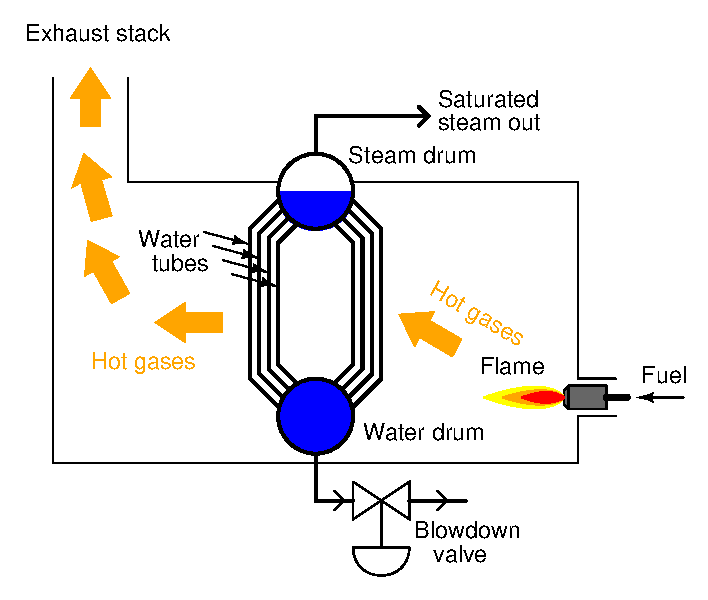
\includegraphics[width=15.5cm]{i01421x01.eps}$$

The engineer who specified this valve was relatively inexperienced, and that inexperience shows in the valve's performance.  Although the valve's C$_{v}$ has been sized appropriately for the pressure drop across it and the density of the hot water flowing through it, it is found that the valve flows {\it much} less water through it than what was expected.  When fully open, the blowdown valve only releases a small fraction of the intended flow rate of water, even when the downstream side is vented to the atmosphere, and the full pressure of the boiler is dropped across the valve.

What is wrong here?  What is preventing the blowdown valve from flowing enough water when wide-open?
 
\underbar{file i01421}
%(END_QUESTION)





%(BEGIN_ANSWER)

The answer to this question (no, I'm not going to just give it away!) relates to the physics of heated, pressurized water.  What happens to a pressurized liquid when it is released into the atmosphere, if the temperature of that liquid is well above its boiling point at atmospheric pressure?
 
%(END_ANSWER)





%(BEGIN_NOTES)

As the hot boiler water enters the valve, it encounters a sharp drop in pressure, and flashes into steam.  The rapid expansion of water to steam results in choking, which severely limits the flow through the valve.

The engineer's error in sizing the valve was to ignore the phase change of water into steam with pressure drop.  Either the valve must be sized larger, or the downstream pressure ($P_2$) raised, in order to eliminate this problem.

%INDEX% Final Control Elements, valve: choked flow
%INDEX% Final Control Elements, valve: sizing
%INDEX% Process: steam boiler blowdown

%(END_NOTES)


